\documentclass[10pt,a4paper]{article}
\usepackage[UTF8,fontset = windows]{ctex}
\setCJKmainfont[BoldFont=黑体,ItalicFont=楷体]{华文中宋}
\usepackage{amssymb,amsmath,amsfonts,amsthm,mathrsfs,dsfont,graphicx}
\usepackage{ifthen,indentfirst,enumerate,color,titletoc}
\usepackage{tikz}
\usetikzlibrary{arrows,calc}
\usepackage[bf,small,indentafter,pagestyles]{titlesec}
\usepackage[top=1in, bottom=1in,left=0.8in,right=0.8in]{geometry}
\renewcommand{\baselinestretch}{1.65}
\newtheorem{defi}{定义~}
\newtheorem{eg}{例~}
\newtheorem{ex}{~}
\newtheorem{rem}{注~}
\newtheorem{thm}{定理~}
\newtheorem{coro}{推论~}
\newtheorem{axiom}{公理~}
\newtheorem{prop}{性质~}

\newcommand{\blank}[1]{\underline{\hbox to #1pt{}}}
\newcommand{\bracket}[1]{(\hbox to #1pt{})}

\begin{document}

\begin{enumerate}[1.]

%赋能1

\item  若``$a>b$'', 则``$a^3>b^3$''是\blank{50}命题(填: 真、假).
\item  已知$A=(-\infty ,0]$, $B=(a,+\infty )$, 若$A\cup B=\mathbf{R}$, 则$a$的取值范围是\blank{50}.
\item  $z+2\bar{z}=9+4\mathrm{i}$($\mathrm{i}$为虚数单位), 则$|z|=$\blank{50}.
\item  若$\triangle ABC$中, $a+b=4$, $\angle C=30^\circ$, 则$\triangle ABC$面积的最大值是\blank{50}.
\item  若函数$f(x)=\log_2\dfrac{x-a}{x+1}$的反函数的图像过点$(-2,3)$, 则$a=$\blank{50}.
\item  若半径为2的球$O$表面上一点$A$作球$O$的截面, 若$OA$与该截面所成的角是$60^\circ$, 则该
截面的面积是\blank{50}.
\item  抛掷一枚均匀的骰子(刻有1、2、3、4、5、6)三次, 得到的数字依次记作$a$、$b$、$c$, 则$a+b\mathrm{i}$($\mathrm{i}$为虚数单位)是方程$x^2-2x+c=0$的根的概率是\blank{50}.
\item  设常数$a>0$, $(x+\dfrac{a}{\sqrt{x}})^9$展开式中$x^6$的系数为$4$, 则$\displaystyle\lim_{n\to \infty}(a+a^2+\cdots+a^n)=$\blank{50}.
\item  已知直线$l$经过点$(-\sqrt{5},0)$且方向向量为$(2,-1)$, 则原点$O$到直线$l$的距离为\blank{50}.
\item  若双曲线的一条渐近线为$x+2y=0$, 且双曲线与抛物线$y=x^2$的准线仅有一个公共点, 则此双曲线的标准方程为\blank{50}.

%赋能2

\item $\displaystyle\lim_{n\to \infty}\dfrac{2n-5}{n+1}=$\blank{50}.
\item 已知抛物线$C$的顶点在平面直角坐标系原点, 焦点在$x$轴上, 若$C$经过点$M(1,3)$, 则其焦点到准线的距离为\blank{50}.
\item 若线性方程组的增广矩阵为$\begin{pmatrix}    a & 0 & 2 \\ 0 & 1 & b\end{pmatrix}$, 解为$\begin{cases}    x=2, \\ y=1.\end{cases}$ 则$a+b=$\blank{50}.
\item 若复数$z$满足: $\mathrm{i}\cdot z=\sqrt{3}+\mathrm{i}$($\mathrm{i}$是虚数单位), 则$|z|=$\blank{50}.
\item 在$(x+\dfrac{2}{x^2})^6$的二项展开式中第四项的系数是\blank{50}(结果用数值表示).
\item 在长方体$ABCD-A_1B_1C_1D_1$中, 若$AB=BC=1$, $AA_1=\sqrt{2}$, 则异面直线$BD_1$与$CC_1$所成角的大小为\blank{50}.
\item 若函数$f(x)=\begin{cases}    2^x, & x\le 0, \\ -x^2+m, & x>0 \end{cases}$的值域为$(-\infty ,1]$, 则实数$m$的取值范围是\blank{50}.
\item 如图, 在$\triangle ABC$中, 若$AB=AC=3$, $\cos \angle BAC=\dfrac{1}{2}$, $\overrightarrow{DC}=2\overrightarrow{BD}$, 则$\overrightarrow{AD}\cdot \overrightarrow{BC}=$\blank{50}.
\begin{center}
    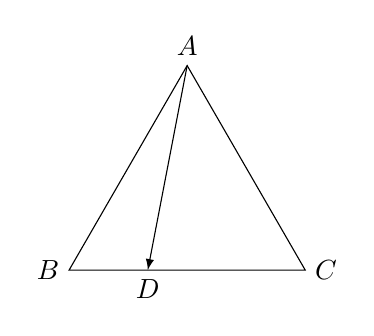
\begin{tikzpicture}[>=latex]
        \draw (0,0) node [left] {$B$} -- (3,0) node [right] {$C$} -- (1.5,{1.5*sqrt(3)}) node [above] {$A$} coordinate (A) -- cycle;
        \draw [->] (A) -- (1,0) node [below] {$D$};
    \end{tikzpicture}
\end{center}
\item 定义在$\mathbf{R}$上的偶函数$y=f(x)$, 当$x\ge 0$时, $f(x)=\lg (x^2-3x+3)$, 则$f(x)$在$\mathbf{R}$上的零点个数为\blank{50}个.
\item 将$6$辆不同的小汽车和$2$辆不同的卡车驶入如图所示的$10$个车位中的某$8$个内, 其中$2$辆卡车必须停在$A$与$B$的位置, 那么不同的停车位置安排共有\blank{50}种(结果用数值表示).
\begin{center}
    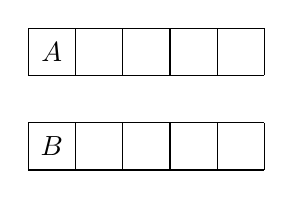
\begin{tikzpicture}[>=latex]
        \draw (0,0) node {$B$};
        \draw (0,1.2) node {$A$};
        \foreach \i in {-0.3,0.3,0.9,1.5}{\draw (-0.3,\i) -- (2.7,\i);};
        \foreach \i in {-0.3,0.3,...,2.8}{\draw (\i,-0.3) -- (\i, 0.3) (\i, 0.9) -- (\i, 1.5);};
    \end{tikzpicture}
\end{center}

% 赋能3 

\item 设集合$A=\{x||x-2|<1,x\in \mathbf{R}\}$, 集合$B=\mathbf{Z}$, 则$A\cap B=$\blank{50}.
\item 函数$y=\sin (\omega x-\dfrac{\pi}{3})$($\omega >0$)的最小正周期是$\pi$, 则$\omega =$\blank{50}.
\item 设$\mathrm{i}$为虚数单位, 在复平面上, 复数$\dfrac{3}{(2-\mathrm{i})^2}$对应的点到原点的距离为\blank{50}.
\item 若函数$f(x)=\log_2 (x+1)+a$的反函数的图像经过点$(4,1)$, 则实数$a=$\blank{50}.
\item 已知$(a+3b)^n$的展开式中, 各项系数的和与各项二项式系数的和之比为$64$, 则$n=$\blank{50}.
\item 甲、乙两人从$5$门不同的选修课中各选修$2$门, 则甲、乙所选的课程中恰有$1$门相同的选法有\blank{50}种.
\item 若圆锥的侧面展开图是半径为2$\text{cm}$, 圆心角为$270^\circ$的扇形, 则这个圆锥的体积为\blank{50}$\text{cm}^3$.
\item 若数列$\{a_n\}$的所有项都是正数, 且$\sqrt{a_1}+\sqrt{a_2}+\cdots +\sqrt{a_n}=n^2+3n$($n\in \mathbf{N}^*$), 则$\displaystyle\lim_{n\to\infty}\dfrac{1}{n^2}(\dfrac{a_1}{2}+\dfrac{a_2}{3}+\cdots +\dfrac{a_n}{n+1})=$\blank{50}.
\item 如图, 在$\triangle ABC$中, $\angle B=45^\circ$, $D$是$BC$边上的一点, $AD=5$, $AC=7$, $DC=3$, 则$AB$的长为\blank{50}.
\begin{center}
    \begin{tikzpicture}[scale = 0.5]
        \draw  (-6.830127018922193,0.)-- (3.,0.) node [below right] {$C$};
        \draw  (3.,0.)-- (-2.5,4.330127018922193) node [above] {$A$};
        \draw  (-2.5,4.330127018922193)-- (-6.830127018922193,0.) node [below left] {$B$};
        \draw  (-2.5,4.330127018922193)-- (0.,0.) node [below] {$D$};
    \end{tikzpicture}
\end{center}
\item 有以下命题:\\
\textcircled{1} 若函数$f(x)$既是奇函数又是偶函数, 则$f(x)$的值域为$\{0\}$; \\
\textcircled{2} 若函数$f(x)$是偶函数, 则$f(|x|)=f(x)$;\\
\textcircled{3} 若函数$f(x)$在其定义域内不是单调函数, 则$f(x)$不存在反函数;\\
\textcircled{4} 若函数$f(x)$存在反函数${{f}^{-1}}(x)$, 且${{f}^{-1}}(x)$与$f(x)$不完全相同, 则$f(x)$与${{f}^{-1}}(x)$图像的公共点必在直线$y=x$上; \\
其中真命题的序号是\blank{50}(写出所有真命题的序号).

% 赋能4

\item 若集合$A=\{x|y^2=x,y\in \mathbf{R}\}$, $B=\{y|y=\sin x,x\in \mathbf{R}\}$, 则$A\cap B=$\blank{50}.
\item 若$-\dfrac{\pi}{2}<\alpha <\dfrac{\pi}{2}$, $\sin \alpha =\dfrac{3}{5}$, 则$\cot 2\alpha =$\blank{50}.
\item 函数$f(x)=1+\log_2 x$($x\ge 1$)的反函数$f^{-1}(x)=$\blank{50}.
\item 若$(1+x)^5=a_0+a_1x+a_2x^2+\cdots+a_5x^5$, 则$a_1+a_2+\cdots+a_5=$\blank{50}.
\item 设$k\in \mathbf{R}$, $\dfrac{y^2}{k}-\dfrac{x^2}{k-2}=1$表示焦点在$y$轴上的双曲线, 则半焦距的取值范围是\blank{50}.
\item 设$m\in \mathbf{R}$, 若$f(x)=(m+1)x^{\tfrac{2}{3}}+mx+1$是偶函数, 则$f(x)$的单调递增区间是\blank{50}.
\item 方程$\log_2(9^x-5)=2+\log_2(3^x-2)$的解$x=$\blank{50}.
\item 已知圆$C:x^2+y^2+2kx+2y+k^2=0$($k\in \mathbf{R}$)和定点$P(1,-1)$, 若过$P$可以作两条直线与圆$C$相切, 则$k$的取值范围是\blank{50}.
\item 如图, 在直三棱柱$ABC-A_1B_1C_1$中, $\angle ABC=90^\circ$, $AB=BC=1$, 若$A_1C$与平面$B_1BCC_1$所成的角为$\dfrac{\pi}{6}$, 则三棱锥$A_1-ABC$的体积为\blank{50}.
\begin{center}
    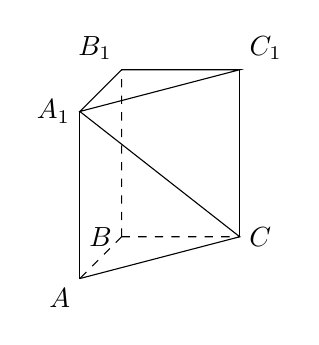
\begin{tikzpicture}[scale = 1.5]
        \draw [dashed] (0,0) -- (1,0) node [right] {$C$} coordinate (C) (0,0) -- (225:0.5) node [below left] {$A$} coordinate (A) (0,0) node [left] {$B$} coordinate (B) -- (0,{sqrt(2)}) node [above left] {$B_1$} coordinate (B1);
        \draw (A) --+ (0,{sqrt(2)}) node [left] {$A_1$} coordinate (A1);
        \draw (C) --+ (0,{sqrt(2)}) node [above right] {$C_1$} coordinate (C1);
        \draw (A1) -- (B1) -- (C1) -- (A1) -- (C) -- (A);
    \end{tikzpicture}
\end{center}
\item 设地球半径为$R$, 若$A$、$B$两地均位于北纬$45^\circ$, 且两地所在纬度圈上的弧长为$\dfrac{\sqrt{2}}{4}\pi R$, 则$A$、$B$之间的球面距离是\blank{50}(结果用含有$R$的代数式表示).

% 赋能5

\item 复数$\mathrm{i}(2+\mathrm{i})$的虚部为\blank{50}.
\item 设函数$f(x)=\begin{cases}\log_2 x, & x>0, \\ 4^x, & x\le 0,\end{cases}$ 则$f(f(-1))=$\blank{50}.
\item 已知$M=\{x||x-1|\le 2,x\in \mathbf{R}\}$, $P=\{x|\dfrac{1-x}{x+2}\ge 0,x\in \mathbf{R}\}$, 则$M\cap P=$\blank{50}.
\item 抛物线$y=x^2$上一点$M$到焦点的距离为$1$, 则点$M$的纵坐标为\blank{50}.
\item 已知无穷数列$\{a_n\}$满足$a_{n+1}=\dfrac12{a_n}$($n\in \mathbf{N}^*$), 且$a_2=1$, 记$S_n$为数列$\{a_n\}$的前$n$项和, 则$\displaystyle\lim_{n\to \infty}S_n=$\blank{50}.
\item 已知$x,y\in \mathbf{R}^+$, 且$x+2y=1$, 则$xy$的最大值为\blank{50}.
\item 已知圆锥的母线$l=10$, 母线与旋转轴的夹角$\alpha =30^\circ$, 则圆锥的表面积为\blank{50}.
\item 若$(2x^2+\dfrac1x)^n$($n\in \mathbf{N}^*$)的二项展开式中的第$9$项是常数项, 则$n=$\blank{50}.
\item 已知$A,B$分别是函数$f(x)=2\sin \omega x$($\omega >0$)在$y$轴右侧图像上的第一个最高点和第一个最低点, 且$\angle AOB=\dfrac\pi 2$, 则该函数的最小正周期是\blank{50}.
\item 将序号分别为1、2、3、4、5的$5$张参观券全部分给$4$人, 每人至少一张, 如果分给同一人的$2$张参观券连号, 那么不同的分法种数是\blank{50}.

% 赋能6

\item $\displaystyle\lim_{n\to\infty}\dfrac{2n+3}{n+1}=$\blank{50}.
\item 设全集$U=\mathbf{R}$, 集合$A=\{-1,0,1,2,3\}$, $B=\{x|x\ge 2\}$, 则$A\cap {\complement_U}B=$\blank{50}.
\item 不等式$\dfrac{x+1}{x+2}<0$的解集为\blank{50}.
\item 椭圆$\begin{cases} x=5\cos \theta,  \\ y=4\sin \theta  \end{cases}$($\theta$为参数)的焦距为\blank{50}.
\item 若函数$y=\begin{vmatrix}   \cos x & \sin x  \\   \sin x & \cos x  \\ \end{vmatrix}$的最小正周期为$a\pi $, 则实数$a$的值为\blank{50}.
\item 若点$(8,4)$在函数$f(x)=1+\log_a x$图像上, 则$f(x)$的反函数为\blank{50}.
\item 已知向量$\overrightarrow{a}=(1,2)$, $\overrightarrow{b}=(0,3)$, 则$\overrightarrow{b}$在$\overrightarrow{a}$的方向上的投影为\blank{50}.
\item 已知一个底面置于水平面上的圆锥, 其左视图是边长为6的正三角形, 则该圆锥的侧面积为\blank{50}.
\item 某班级要从$5$名男生和$2$名女生中选出$3$人参加公益活动, 则在选出的$3$人中男、女生
均有的概率为\blank{50}(结果用最简分数表示).
\item 设常数$a>0$, 若$(x+\dfrac ax)^9$的二项展开式中$x^5$的系数为$144$, 则$a=$\blank{50}.

% 赋能7

\item 设集合$M=\{x|x^2=x\}$, $N=\{x|\lg x\le 0\}$, 则$M\cap N=$\blank{50}.
\item 已知$a$、$b\in \mathbf{R}$, $\mathrm{i}$是虚数单位, 若$a+\mathrm{i}=2-b\mathrm{i}$, 则$(a+b\mathrm{i})^2=$\blank{50}.
\item 已知函数$f(x)=a^x-1$的图像经过$(1,1)$点, 则$f^{-1}(3)=$\blank{50}.
\item 不等式$x|x-1|>0$的解集为\blank{50}.
\item 已知$\overrightarrow a=(\sin x,\cos x)$, $\overrightarrow b=(\sin x,\sin x)$, 则函数$f(x)=\overrightarrow a\cdot \overrightarrow b$的最小正周期为\blank{50}.
\item 里约奥运会游泳小组赛采用抽签方法决定运动员比赛的泳道, 在由$2$名中国运动员和$6$名外国运动员组成的小组中, $2$名中国运动员恰好抽在相邻泳道的概率为\blank{50}.
\item 如图, 在棱长为$1$的正方体$ABCD-A_1B_1C_1D_1$中, 点$P$在截面$A_1DB$上, 则线段$AP$的最小值为\blank{50}.
\begin{center}
    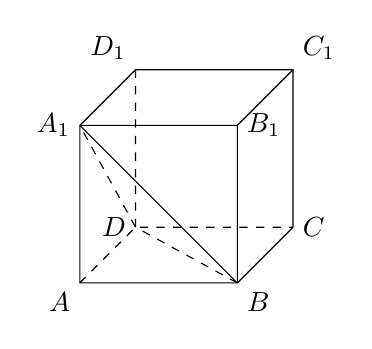
\begin{tikzpicture}
        \draw (0,0) node [below left] {$A$} coordinate (A) --++ (2,0) node [below right] {$B$} coordinate (B) --++ (45:{2/2}) node [right] {$C$} coordinate (C)
        --++ (0,2) node [above right] {$C_1$} coordinate (C1)
        --++ (-2,0) node [above left] {$D_1$} coordinate (D1) --++ (225:{2/2}) node [left] {$A_1$} coordinate (A1) -- cycle;
        \draw (A) ++ (2,2) node [right] {$B_1$} coordinate (B1) -- (B) (B1) --++ (45:{2/2}) (B1) --++ (-2,0);
        \draw [dashed] (A) --++ (45:{2/2}) node [left] {$D$} coordinate (D) --++ (2,0) (D) --++ (0,2);
        \draw (A1) -- (B);
        \draw [dashed] (B) -- (D) -- (A1);
    \end{tikzpicture}
\end{center}
\item 设$(1+x)^n=a_0+a_1x+a_2x^2+a_3x^3+\cdots +a_nx^n$, 若$\dfrac{a_2}{a_3}=\dfrac13$, 则$n=$\blank{50}.
\item 已知圆锥底面半径与球的半径都是$1\text{cm}$, 如果圆锥的体积与球的体积恰好也相等, 那么这个圆锥的侧面积是\blank{50}$\text{cm}^2$.
\item 设$P(x,y)$是曲线$C:\sqrt{\dfrac{x^2}{25}}+\sqrt{\dfrac{y^2}9}=1$上的点, $F_1(-4,0)$, $F_2(4,0)$, 则$|PF_1|+|PF_2|$的最大值为\blank{50}.

% 赋能8

\item 已知复数$z=2+\mathrm{i}$($\mathrm{i}$为虚数单位), 则$\overline{{z^2}}=$\blank{50}.
\item 已知集合$A=\{x|\dfrac12\le {2^x}<16\}$, $B=\{x|y=\log _2(9-x^2)\}$, 则$A\cap B=$\blank{50}。
\item 在二项式$(x+\dfrac2x)^6$的展开式中, 常数项是\blank{50}.
\item 等轴双曲线$x^2-y^2=a^2$与抛物线$y^2=16x$的准线交于$A$、$B$两点, 且$|AB|=4\sqrt3$, 则该双曲线的实轴长等于\blank{50}.
\item 若由矩阵$\begin{pmatrix}a & 2 \\ 2 & a\end{pmatrix}\begin{pmatrix}x \\ y\end{pmatrix}=\begin{pmatrix}a+2 \\ 2a\end{pmatrix}$表示$x$、$y$的二元一次方程组无解, 则实数$a=$\blank{50}.
\item 已知$f(x)=\sin\dfrac\pi 3x$, $A=\{1,2,3,4,5,6,7,8\}$, 现从集合$A$中任取两个不同元素$s$、$t$, 则使得$f(s)\cdot f(t)=0$发生的概率是\blank{50}.
\item 若圆锥侧面积为$20\pi$, 且母线与底面所成角为$\arccos \dfrac45$, 则该圆锥的体积为\blank{50}.
\item 已知数列$\{a_n\}$的通项公式为$a_n=n^2+bn$, 若数列$\{a_n\}$是单调递增数列, 则实数$b$的取值范围是\blank{50}.
\item 将边长为$10$的正三角形$ABC$, 按``斜二测''画法在水平放置的平面上画出为$\triangle A'B'C'$, 则$\triangle A'B'C'$中最短边的边长为\blank{50}(精确到0.01).
\item 已知点$A$是圆$O: x^2+y^2=4$上的一个定点, 点$B$是圆$O$上的一个动点, 若满足$|\overrightarrow{AO}+\overrightarrow{BO}|=|\overrightarrow{AO}-\overrightarrow{BO}|$, 则$\overrightarrow{AO}\cdot \overrightarrow{AB}=$\blank{50}.

% 赋能9

\item 方程$\lg (3x+4)=1$的解$x=$\blank{50}.
\item 若关于$x$的不等式$\dfrac{x-a}{x-b}>0$($a,b\in \mathbf{R}$)的解集为$(-\infty ,1)\cup (4,+\infty)$, 则$a+b=$\blank{50}.
\item 已知数列$\{a_n\}$的前$n$项和为$S_n=2^n-1$, 则此数列的通项公式为\blank{50}.
\item 函数$f(x)=\sqrt x+1$的反函数是\blank{50}.
\item $(1+2x)^6$展开式中$x^3$项的系数为\blank{50}(用数字作答).
\item 如图, 已知正方形$ABCD-A_1B_1C_1D_1$, $AA_1=2$, $E$为棱$CC_1$的中点, 则三棱锥$D_1-ADE$的体积为\blank{50}.
\begin{center}
    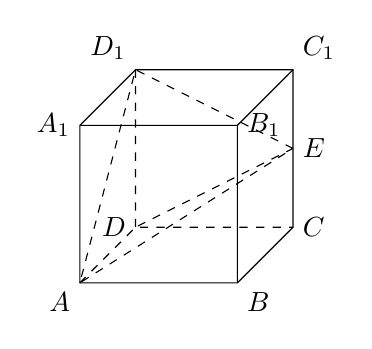
\begin{tikzpicture}
        \draw (0,0) node [below left] {$A$} coordinate (A) --++ (2,0) node [below right] {$B$} coordinate (B) --++ (45:{2/2}) node [right] {$C$} coordinate (C)
        --++ (0,2) node [above right] {$C_1$} coordinate (C1)
        --++ (-2,0) node [above left] {$D_1$} coordinate (D1) --++ (225:{2/2}) node [left] {$A_1$} coordinate (A1) -- cycle;
        \draw (A) ++ (2,2) node [right] {$B_1$} coordinate (B1) -- (B) (B1) --++ (45:{2/2}) (B1) --++ (-2,0);
        \draw [dashed] (A) --++ (45:{2/2}) node [left] {$D$} coordinate (D) --++ (2,0) (D) --++ (0,2);
        \draw ($ (C)!0.5!(C1) $) node [right] {$E$} coordinate (E);
        \draw [dashed] (E) -- (D1) -- (A) -- (E) -- (D);
    \end{tikzpicture}
\end{center}
\item 从单词``shadow''中任意选取$4$个不同的字母排成一排, 则其中含有``a''的共有\blank{50}种排法(用数字作答).
\item 集合$\{x|\cos (\pi \cos x)=0,x\in [0,\pi]\}=$\blank{50}(用列举法表示).
\item 如图, 已知半径为1的扇形$AOB$, $\angle AOB=60^\circ$, $P$为弧$\overset\frown{AB}$上的一个动点, 则$\overrightarrow{OP}\cdot \overrightarrow{AB}$取值范围是\blank{50}.
\begin{center}
    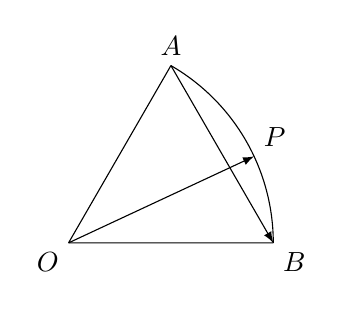
\begin{tikzpicture}[>=latex,scale = 1.3]
        \draw (0,0) node [below left] {$O$} -- (2,0) node [below right] {$B$} (0,0) -- (1,{sqrt(3)}) node [above] {$A$} -- cycle;
        \draw (2,0) arc (0:60:2);
        \draw [->] (0,0) -- (25:2) node [above right] {$P$};
        \draw [->] (1,{sqrt(3)}) -- (2,0);
    \end{tikzpicture}
\end{center}
\item 已知$x$、$y$满足曲线方程$x^2+\dfrac1{y^2}=2$, 则$x^2+y^2$的取值范围是\blank{50}.

% 赋能10

\item 已知$U=\mathbf{R}$, 集合$A=\{x|4-2x\ge x+1\}$, 则${\complement_U}A=$\blank{50}.
\item 三阶行列式$\begin{vmatrix}   3 & -5 & 1 \\   2 & 3 & -6 \\   -7 & 2 & 4 \\ \end{vmatrix}$中元素$-5$的代数余子式的值为\blank{50}.
\item $(1-\dfrac x2)^8$的二项展开式中含$x^2$项的系数是\blank{50}.
\item 已知一个球的表面积为$16\pi$, 则它的体积为\blank{50}.
\item 一个袋子中共有$6$个球, 其中$4$个红色球, $2$个蓝色球, 这些球的质地和形状一样, 从中任意抽取$2$个球, 则所抽的球都是红色球的概率是\blank{50}.
\item 已知直线$l:x-y+b=0$被圆$C:x^2+y^2=25$所截得的弦长为$6$, 则$b=$\blank{50}.
\item 若复数$(1+a\mathrm{i})(2-\mathrm{i})$在复平面上所对应的点在直线$y=x$上, 则实数$a=$\blank{50}.
\item 函数$f(x)=(\sqrt3\sin x+\cos x)(\sqrt3\cos x-\sin x)$的最小正周期为\blank{50}.
\item 过双曲线$C:\dfrac{x^2}{a^2}-\dfrac{y^2}4=1$的右焦点$F$作一条垂直于$x$轴的垂线交双曲线$C$的两条渐近线于$A$、$B$两点, $O$为坐标原点, 则$\triangle OAB$的面积的最小值为\blank{50}.
\item 若关于$x$的不等式$|2^x-m|-\dfrac1{2^x}<0$在区间$[0,1]$内恒成立, 则实数$m$的范围\blank{50}.

% 赋能11

\item 已知集合$A=\{1,2,4,6,8\}$, $B=\{x|x=2k,k\in A\}$, 则$A\cap B=$\blank{50}.
\item 已知$\dfrac{\overline z}{1-\mathrm{i}}=2+\mathrm{i}$, 则复数$z$的虚部为\blank{50}.
\item 设函数$f(x)=\sin x-\cos x$, 且$f(a)=1$, 则$\sin 2a=$\blank{50}.
\item 已知二元一次方程$\begin{cases} {a_1}x+{b_1}y={c_1}, \\  {a_2}x+{b_2}y={c_2} \end{cases}$的增广矩阵是$\begin{pmatrix} 1 & -1 & 1 \\  1 & 1 & 3 \\ \end{pmatrix}$, 则此方程组的解是\blank{50}.
\item 数列$\{a_n\}$是首项为$1$, 公差为$2$的等差数列, $S_n$是它前$n$项和, 则$\displaystyle\lim_{n\to\infty}\dfrac{S_n}{a_n^2}=$\blank{50}.
\item 已知角$A$是$\triangle ABC$的内角, 则``$\cos A=\dfrac12$''是``$\sin A=\dfrac{\sqrt3}2$''的\blank{50}条件(填``充分非必要''、``必要非充分''、``充要条件''、``既非充分又非必要''之一).
\item 若双曲线$x^2-\dfrac{y^2}{b^2}=1$的一个焦点到其渐近线距离为$2\sqrt2$, 则该双曲线焦距等于\blank{50}.
\item 若正项等比数列$\{a_n\}$满足: $a_3+a_5=4$, 则$a_4$的最大值为\blank{50}.
\item 已知函数$f(x)=\sin (2x+\dfrac\pi 3)$在区间$[0,a]$(其中$a>0$)上单调递增, 则实数$a$的取值范围是\blank{50}.
\item 设函数$f(x)=\begin{cases}    x^6, & x\ge 1,  \\   -2x-1, & x\le -1, \end{cases}$ 则当$x\le -1$时, $f[f(x)]$表达式的展开式中含${x^2}$项的系数是\blank{50}.

% 赋能12

\item ``$x<0$''是``$x<a$''的充分非必要条件, 则$a$的取值范围是\blank{50}.
\item 函数$f(x)=1-3\sin ^2(x+\dfrac\pi 4)$的最小正周期为\blank{50}.
\item 若复数$z$为纯虚数, 且满足$(2-\mathrm{i})z=a+\mathrm{i}$($\mathrm{i}$为虚数单位), 则实数$a$的值为\blank{50}.
\item 二项式$(x^2+\dfrac 1x)^5$的展开式中, $x$的系数为\blank{50}.
\item 用半径$1$米的半圆形薄铁皮制作圆锥型无盖容器, 其容积为\blank{50}立方米.
\item 已知$\alpha$为锐角, 且$\cos (\alpha +\dfrac\pi 4)=\dfrac35$, 则$\sin \alpha =$\blank{50}.
\item 已知正四棱柱$ABCD-A_1B_1C_1D_1$, $AB=a$, $AA_1=2a$, $E$、$F$分别是棱$AD$、$CD$的中点,则异面直线$BC_1$与$EF$所成角是\blank{50}.
\item 在无穷等比数列$\{a_n\}$中, $\displaystyle\lim_{n\to\infty}(a_1+a_2+\cdots+a_n)=\dfrac12$, 则$a_1$的取值范围是\blank{50}.
\item 某班班会准备从含甲、乙的$6$名学生中选取$4$人发言, 要求甲、乙两人至少有一人参加, 那么不同的发言顺序有\blank{50}种.
\item 已知奇函数$f(x)$是定义在$\mathbf{R}$上的增函数, 数列$\{x_n\}$是一个公差为$2$的等差数列, 满足$f(x_7)+f(x_8)=0$, 则$x_{2017}$的值为\blank{50}.

% 赋能13

\item 若集合$M=\{x|{x^2}-2x<0\}$, $N=\{x||x|>1\}$, 则$M\cap N=$\blank{50}.
\item 若复数$\angle OFA+\angle OFB={180^\circ}$满足$2z+\overline z=3-2\mathrm{i}$, 其中$\mathrm{i}$为虚数单位, 则$z=$\blank{50}.
\item 如果$\sin \alpha =-\dfrac5{13}$, 且$\alpha$为第四象限角, 则$\tan \alpha$的值是\blank{50}.
\item 函数$f(x)=\begin{vmatrix}   \cos x & \sin x  \\    \sin x & \cos x \end{vmatrix}$的最小正周期是\blank{50}.
\item 函数$f(x)=2^x+m$的反函数为$y=f^{-1}(x)$, 且$y=f^{-1}(x)$的图像过点$Q(5,2)$, 那么$m=$\blank{50}.
\item 点$(1,0)$到双曲线$\dfrac{x^2}4-y^2=1$的渐近线的距离是\blank{50}.
\item 如果实数$x$、$y$满足$\begin{cases} 2x-y\le 0, \\ x+y\le 3, \\  x\ge 0, \\ \end{cases}$, 则$2x+y$的最大值是\blank{50}.
\item 从$5$名学生中任选$3$人分别担任语文、数学、英语课代表, 其中学生甲不能担任数学课代表, 共有\blank{50}种不同的选法(结果用数值表示).
\item 方程$x^2+y^2-4tx-2ty+3t^2-4=0$($t$为参数)所表示的圆的圆心轨迹方程是\blank{50}(结果化为普通方程).
\item 若$a_n$是$(2+x)^n$($n\in \mathbf{N}^*$, $n\ge 2$, $x\in \mathbf{R}$)展开式中$x^2$项的二项式系数, 则$\displaystyle\lim_{n\to\infty}(\dfrac 1{a_2}+\dfrac 1{a_3}+\cdots+\dfrac1{a_n})=$\blank{50}.

% 赋能14

\item 设集合$A=\{2,3,4,12\}$, $B=\{0,1,2,3\}$, 则$A\cap B=$\blank{50}.
\item $\displaystyle\lim_{n\to\infty}\dfrac{5^n-7^n}{5^n+7^n}=$\blank{50}.
\item 函数$y=2\cos^2(3\pi x)-1$的最小正周期为\blank{50}.
\item 不等式$\dfrac{x+2}{x+1}>1$的解集为\blank{50}.
\item 若$z=\dfrac{-2+3\mathrm{i}}{\mathrm{i}}$(其中$\mathrm{i}$为虚数单位), 则$\mathrm{Im} z=$\blank{50}.
\item 若从五个数$-1,0,1,2,3$中任选一个数$m$, 则使得函数$f(x)=(m^2-1)x+1$在$\mathbf{R}$上单调递增的概率为\blank{50}(结果用最简分数表示).
\item 在$(\dfrac3{x^2}+\sqrt{x})^n$的二项展开式中, 所有项的二项式系数之和为$1024$, 则常数项的值等于\blank{50}.
\item 半径为$4$的圆内接三角形$ABC$的面积是$\dfrac1{16}$, 角$A,B,C$所对应的边依次为$a,b,c$, 则$abc$的值为\blank{50}.
\item 已知抛物线$C$的顶点为坐标原点, 双曲线$\dfrac{x^2}{25}-\dfrac{y^2}{144}=1$的右焦点是$C$的焦点$F$. 若斜率为$-1$, 且过$F$的直线与$C$交于$A,B$两点, 则$|AB|=$\blank{50}.
\item 直角坐标系$xOy$内有点$P(-2,-1)$, $Q(0,-2)$, 将$\triangle POQ$绕$x$轴旋转一周, 则所得几何体的体积为\blank{50}.

% 赋能15

\item 已知集合$A=\{1,2,5\}$, $B=\{2,a\}$. 若$A\cup B=\{1,2,3,5\}$, 则$a=$\blank{50}.
\item 抛物线$y^2=4x$的焦点坐标是\blank{50}.
\item 不等式$\dfrac x{x+1}<0$的解是\blank{50}.
\item 若复数$z$满足$\mathrm{i}z=1+\mathrm{i}$($\mathrm{i}$为虚数单位), 则$z=$\blank{50}.
\item 在代数式$(x+\dfrac 1{x^2})^7$的展开式中, 一次项的系数是\blank{50}(用数字作答).
\item 若函数$y=2\sin (\omega x-\dfrac\pi 3)+1 \ (\omega >0)$的最小正周期是$\pi$, 则$\omega=$\blank{50}.
\item 若函数$f(x)=x^a$的反函数的图像经过点$(\dfrac12,\dfrac14)$, 则$a=$\blank{50}.
\item 将一个正方形绕着它的一边所在的直线旋转一周, 所得几何体的体积为$27\pi\text{cm}^3$, 则该几何体的侧面积为\blank{50}$\text{cm}^3$.
\item 已知函数$y=f(x)$是奇函数, 当$x<0$时, $f(x)=2^x-ax$, 且$f(2)=2$, 则$a=$\blank{50}.
\item 若无穷等比数列$\{a_n\}$的各项和为$S_n$, 首项$a_1=1$, 公比为$a-\dfrac32$, 且$\displaystyle\lim_{n\to\infty}S_n=a$, 则$a=$\blank{50}.

% 赋能16

\item 已知全集$U=\mathbf{N}$, 集合$A=\{1,2,3,4\}$, 集合$B=\{3,4,5\}$, 则$(\complement_U A)\cap B=$\blank{50}.
\item 复数$\dfrac2{1+\mathrm{i}}$的虚部是\blank{50}.
\item 用$1,2,3,4,5$共$5$个数排成一个没有重复数字的三位数, 则这样的三位数有\blank{50}个.
\item 已知$\tan \theta =-2$, 且$\theta \in (\dfrac\pi 2,\pi)$, 则$\cos\theta=$\blank{50}.
\item 圆锥的底面半径为$1$, 母线长为$3$, 则圆锥的侧面积等于\blank{50}.
\item 已知向量$\overrightarrow{a}=(1,\sqrt{3})$, $\overrightarrow{b}=(3,m)$. 若向量$\overrightarrow{b}$在$\overrightarrow{a}$方向上的投影为$3$, 则实数$m=$\blank{50}.
\item 已知球主视图的面积等于$9\pi$, 则该球的体积为\blank{50}.
\item $(x+\dfrac{1}{x^2})^9$的二项展开式中, 常数项的值为\blank{50}.
\item 已知$A(2,0)$, $B(4,0)$, 动点$P$满足$|PA|=\dfrac{\sqrt2} 2|PB|$, 则$P$到原点的距离为\blank{50}.
\item 设焦点为$F_1$、$F_2$的椭圆$\dfrac{x^2}{a^2}+\dfrac{y^2}3=1 \ (a>0)$上的一点$P$也在抛物线$y^2=\dfrac94x$上, 抛物线焦点为$F_3$, 若$|PF_3|=\dfrac{25}{16}$, 则$\triangle PF_1F_2$的面积为\blank{50}.

% 赋能58

\item 设集合$M=\{x|x^2=x\}$, $N=\{x|\log_2 x\le 0\}$, 则$M\cup N=$\blank{50}.
\item 已知虚数$1+2\mathrm{i}$是方程$x^2+ax+b=0 (a\,b\in \mathbf{R})$的一个根, 则$a+b=$\blank{50}.
\item 在报名的$5$名男生和$4$名女生中, 选取$5$人参加志愿者服务, 要求男、女生都有, 则不同的选取方式的种数为\blank{50}(结果用数值表示).
\item 已知复数$z$在复平面上对应的点在曲线$y=\dfrac 2 x$上运动, 则$|z|$的最小值等于\blank{50}.
\item 在正项等比数列$\{a_n\}$中, $a_1a_3=1$, $a_2+a_3=\dfrac43$, 则$\displaystyle\lim_{n\to\infty}(a_1+a_2+\cdots +a_n)=$\blank{50}.
\item 已知$f(x)=2 \sin \omega x\ (\omega >0)$在$[0,\dfrac\pi 3]$单调递增, 则实数$\omega$的最大值为\blank{50}.
\item 若行列式$\begin{vmatrix}   1 & 2 & 4 \\   \cos (\pi +x) & 2 & 0 \\   -1 & 1 & 6 \end{vmatrix}$中的元素$4$的代数余子式的值等于$\dfrac32$, 则实数$x$的取值集合为\blank{50}.
\item 若二项式$(2x-\dfrac1{\sqrt x})^n$展开式中的第$5$项为常数项, 则展开式中各项的二项式系数之和为\blank{50}. 
\item 已知$A$、$B$是球$O$的球面上两点, $\angle AOB=90^\circ$, $C$为该球面上的动点, 若三棱锥$O-ABC$体积的最大值为$\dfrac{32}{3}$, 则球$O$的表面积为\blank{50}.
\begin{center}
    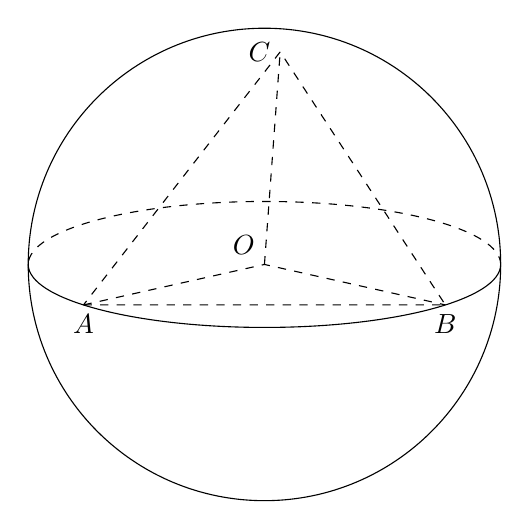
\begin{tikzpicture}
        \draw (0,0) circle (3);
        \draw (-3,0) arc (180:360:3 and 0.8);
        \draw [dashed] (3,0) arc (0:180:3 and 0.8);
        \draw ({3*cos(-140)},{0.8*sin(-140)}) coordinate (A) node [below] {$A$};
        \draw ({3*cos(-40)},{0.8*sin(-40)}) coordinate (B) node [below] {$B$};
        \draw (0.2,2.7) coordinate (C) node [left] {$C$};
        \draw (0,0) coordinate (O) node [above left] {$O$};
        \draw [dashed] (A) -- (B) -- (C) -- cycle;
        \draw [dashed] (A) -- (O) -- (B) (O) -- (C);
    \end{tikzpicture}
\end{center}
\item 如图, $A$、$B$为椭圆$\dfrac{x^2}{a^2}+\dfrac{y^2}{b^2}=1 \ (a>b>0)$的两个顶点, 过椭圆的右焦点$F$作$x$轴的垂线, 与其交于点$C$. 若$AB\parallel OC$($O$为坐标原点), 则直线$AB$的斜率为\blank{50}. 
\begin{center}
    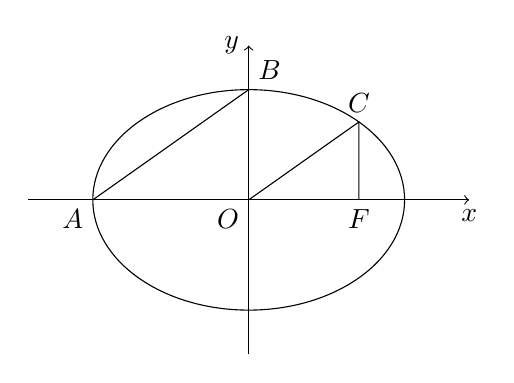
\begin{tikzpicture}[scale = 1.4]
        \draw [->] (-2,0) -- (2,0) node [below] {$x$};
        \draw [->] (0,-1.4) -- (0,1.4) node [left] {$y$};
        \draw (0,0) node [below left] {$O$};
        \draw (0,0) ellipse ({sqrt(2)} and 1);
        \draw (1,0) node [below] {$F$} -- (1,{sqrt(2)/2}) node [above] {$C$} -- (0,0);
        \draw ({-sqrt(2)},0) node [below left] {$A$} -- (0,1) node [above right] {$B$};
    \end{tikzpicture}
\end{center}
\item 若经过抛物线 $y^2=4x$焦点的直线$l$与圆$(x-4)^2+y^2=4$相切, 则直线$l$的方程为\blank{50}.

% 赋能59

\item 若集合$A=\{x|y=\sqrt{x-1},\ x\in \mathbf{R}\}$, $B=\{x||x|\le 1,\ x\in \mathbf{R}\}$, 则$A\cap B=$\blank{50}.
\item 若函数$f(x)=1+\dfrac1x$($x>0$)的反函数为$f^{-1}(x)$, 则不等式$f^{-1}(x)>2$的解集为\blank{50}.
\item 若$\sin \alpha =\dfrac35$且$\alpha$是第二象限角, 则$\tan(\alpha -\dfrac\pi 4)=$\blank{50}.
\item 若函数$f(x)$是定义在$\mathbf{R}$上的奇函数, 且满足$f(x+2)=-f(x)$, 则$f(2016)=$\blank{50}.
\item 在$(x^3-\dfrac1x)^8$的展开式中, 其常数项的值为\blank{50}.
\item 若函数$f(x)=\sin 2x$, $g(x)=f(x+\dfrac\pi 6)$, 则函数$g(x)$的单调递增区间为\blank{50}.
\item 设$P$是曲线$\begin{cases} x=\dfrac{\sqrt2}2\sec \theta, \\ y=\tan \theta \end{cases}$($\theta $为参数)上的一动点, $O$为坐标原点, $M$为线段$OP$的中点, 则点$M$的轨迹的普通方程为\blank{50}.
\item 不等式组$\begin{cases} x\le 3, \\ x+y\ge 0, \\ x-y+2 \ge 0 \end{cases}$所表示的区域的面积为\blank{50}.
\item 若函数$f(x)=\log _5 x$($x>0$), 则方程$f(x+1)+f(x-3)=1$的解$x=$\blank{50}.
\item 如图所示, 三个边长为$2$的等边三角形有一条边在同一直线上, 边$B_3C_3$上有$10$个不同的点$P_1,P_2,\cdots,P_{10}$, 记$M_i=\overrightarrow{AB_2}\cdot \overrightarrow{AP_i}$($i=1,2,\cdots,10$), 则$M_1+M_2+\cdots+M_{10}=$\blank{50}.
\begin{center}
    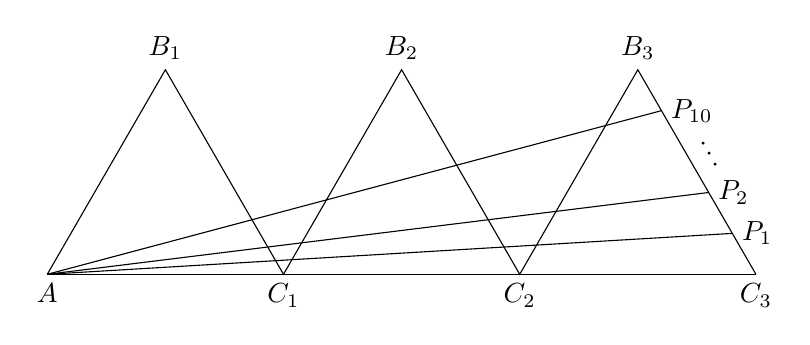
\begin{tikzpicture}[scale = 3]
        \draw (0,0) node [below] {$A$} -- (1,0) node [below] {$C_1$} -- (2,0) node [below] {$C_2$} -- (3,0) node [below] {$C_3$};
        \draw (3,0) -- (2.5,{sqrt(3)/2}) node [above] {$B_3$} -- (2,0) -- (1.5,{sqrt(3)/2}) node [above] {$B_2$} -- (1,0) -- (0.5,{sqrt(3)/2}) node [above] {$B_1$} -- (0,0);
        \draw ($(3,0)!0.2!(2.5,{sqrt(3)/2})$) coordinate (P1) node [right] {$P_1$} -- (0,0);
        \draw ($(3,0)!0.4!(2.5,{sqrt(3)/2})$) coordinate (P2) node [right] {$P_2$} -- (0,0);
        \draw ($(3,0)!0.8!(2.5,{sqrt(3)/2})$) coordinate (P3) node [right] {$P_{10}$} -- (0,0);
        \draw ($(3,0)!0.6!(2.5,{sqrt(3)/2})$) node [right] {\rotatebox{120}{$\cdots$}};
    \end{tikzpicture}
\end{center}

% 赋能60

\item 已知全集$U=\mathbf{R}$, $A=\{x|x^2-2x<0\}$, $B=\{x|x\ge 1\}$, 则$A\cap \complement_U B=$\blank{50}.
\item 若函数$y=\cos ^2 \omega x$($\omega >0$)的最小正周期是$\pi$, 则$\omega=$\blank{50}.
\item 圆$C:x^2+y^2-2x-4y+4=0$的圆心到直线$3x+4y+4=0$的距离$d=$\blank{50}.
\item 已知圆锥的母线长为$5\text{cm}$, 侧面积为$15 \pi \text{cm}^2$, 则此圆锥的体积为\blank{50}$\text{cm}^2$.
\item 已知$x,y\in \mathbf{R}^+$, 且满足$\dfrac x3+\dfrac y4=1$, 则$xy$的最大值为\blank{50}.
\item 已知双曲线$\dfrac{x^2}{a^2}-\dfrac{y^2}{b^2}=1 \ (a>0,\ b>0)$的一条渐近线方程是$y=\sqrt3x$, 它的一个焦点与抛物线$y^2=16x$的焦点相同, 则双曲线的标准方程为\blank{50}.
\item 已知函数$f(x)=\begin{cases}2^x +a, & x\ge 0, \\ x^2-ax, & x<0.\end{cases}$ 若$f(x)$的最小值是$a$, 则$a=$\blank{50}.
\item 从$6$名男医生和$3$名女医生中选出$5$人组成一个医疗小组, 若这个小组中必须男女医生都有, 共有\blank{50}种不同的组建方案(结果用数值表示).
\item 若数列$\{a_n\}$是首项为$1$, 公比为$a-\dfrac32$的无穷等比数列, 且$\{a_n\}$各项的和为$a$, 则$a$的值是\blank{50}.
\item 设$a\ne 0$, $n$是大于$1$的自然数, $(1+\dfrac xa)^n$的展开式为$a_0+a_1x+a_2x^2+\cdots+a_nx^n$. 若$a_1=3$, $a_2=4$, 则$a=$\blank{50}.
\item 矩形$ABCD$中, $AB=2$, $AD=1$, $P$为矩形内部一点, 且$AP=1$. 若$\overrightarrow{AP}=\lambda \overrightarrow{AB}+\mu \overrightarrow{AD} \ (\lambda,\ \mu \in \mathbf{R})$, 则$2 \lambda +\sqrt3\mu$的最大值是\blank{50}.

% 赋能61

\item 函数$y=\log_3 (x-1)$的定义域是\blank{50}.
\item 集合$A=\{x|x^2-3x<0\}$, $B=\{x||x|<2\}$, 则$A\cup B$等于\blank{50}.
\item 若复数$\dfrac{1+\mathrm{i}}{1-\mathrm{i}}+\dfrac12b$($\mathrm{i}$为虚数单位)的实部与虚部相等, 则实数$b$的值为\blank{50}.
\item 已知函数$f(x)=\begin{vmatrix}   {\log _3}x & 1  \\   2 & 1  \\\end{vmatrix}$, 则$f^{-1}(0)=$\blank{50}.
\item 若一个圆锥的母线长是底面半径的$3$倍, 则该圆锥的侧面积是底面积的\blank{50}倍.
\item 平面向量$\overrightarrow a$与$\overrightarrow b$的夹角为$60^\circ$, $|\overrightarrow a|=1$, $\overrightarrow b=(3,0)$, 则$|2 \overrightarrow a+\overrightarrow b|=$\blank{50}.
\item 已知$\triangle ABC$的周长为$4$, 且$\sin A+\sin B=3 \sin C$, 则$AB$边的长为\blank{50}.
\item 若$a_n$为$(1+x)^n$的展开式中的$x^2$项的系数, 则$\displaystyle\lim_{n\to\infty}\dfrac{2a_n}{n^2+1}=$\blank{50}.
\item 若$m>0$, $n>0$, $m+n=1$, 且$\dfrac t m+\dfrac 1 n$($t>0$)的最小值为$9$, 则$t=$\blank{50}.
\item 若以$x$轴正方向为始边, 曲线上的点与圆心的连线为终边的角$\theta$为参数, 则圆$x^2+y^2-2x=0$的参数方程为\blank{50}.
\item 若$AB$是圆$x^2+(y-3)^2=1$的任意一条直径, $O$为坐标原点, 则$\overrightarrow{OA}\cdot \overrightarrow{OB}$的值为\blank{50}.

% 赋能62

\item 已知集合$A=\{-1,3,2m-1\}$, 集合$B=\{3,m^2\}$. 若$B\subseteq A$, 则实数$m=$\blank{50}.  
\item 计算: $\displaystyle\lim_{n\to\infty}\dfrac{3^n+1}{3^{n+1}+2^n}=$\blank{50}.  
\item 函数$f(x)=\sqrt[3]x+1$的反函数$f^{-1}(x)=$\blank{50}.  
\item 函数$f(x)=(\sin x-\cos x)^2$的最小正周期为\blank{50}.  
\item 直线$x+2y-1=0$与直线$y=1$的夹角大小为\blank{50}(结果用反三角函数值表示).
\item 已知菱形$ABCD$, 若$|\overrightarrow{AB}|=1$, $A=\dfrac\pi 3$, 则向量$\overrightarrow{AC}$在$\overrightarrow{AB}$上的投影为\blank{50}.  
\item 已知一个凸多面体的平面展开图由两个正六边形和六个正方形构成, 如图所示, 若该凸多面体所有棱长均为$1$, 则其体积$V=$\blank{50}.
\begin{center}
    \begin{tikzpicture}[scale = 0.6]
        \draw (0,0) -- (6,0) (0,1) -- (6,1);
        \foreach \i in {0,1,...,6}{\draw (\i,0) -- (\i,1);};
        \draw (1,1) --++ (60:1) --++ (120:1) --++ (180:1) --++ (240:1) --++ (300:1); 
        \draw (6,0) --++ (-60:1) --++ (-120:1) --++ (-180:1) --++ (-240:1) --++ (-300:1);
    \end{tikzpicture}
\end{center}
\item 已知函数$f(x)={x^3}+\lg (\sqrt{x^2+1}+x)$, 若$f(x)$的定义域中的$a$、$b$满足$f(-a)+f(-b)-3=f(a)+f(b)+3$, 则$f(a)+f(b)=$\blank{50}.  
\item 数列$\{a_n\}$中, 若$a_1=3$, $\sqrt{a_{n+1}}=a_n$($n\in \mathbf{N}^*$), 则数列$\{a_n\}$的通项公式$a_n=$\blank{50}.
\item 在代数式$(4x^2-2x-5)(1+\dfrac1{x^2})^5$的展开式中, 常数等于\blank{50}.  
\item 满足约束条件$|x|+2|y|\le 2 $的目标函数$z=y-x$的最大值是\blank{50}.

% 赋能63

\item 123


\end{enumerate}

\end{document}